\section{The microcanonical ensemble}\label{sec:MicroCan}
The first statistical approach to the study of a thermodynamic system is the \textbf{microcanonical ensemble}. The systems we will study are \textbf{perfectly isolated} and thus characterized by fixed energy, volume and amount of matter. \\ In phase space, such systems will evolve on surfaces of constant energy $\mathcal{H} (q_i,p_i)=E$. We will define a probability distribution on phase space, such that $\rho(q_i,p_i)dpdq$ will be the probability of finding the system in the microstate $(q_i,p_i)$.\\

The microcanonical probability distribution is built on the assumption of \textbf{a priori uniform probability} on the surface of constant energy $S_E$. In this way the probability distribution reads:
\begin{equation}
    \label{MicroCanPDF}
    \rho_{mc}(q_i,p_i)=\frac{\delta(\mathcal{H} -E)}{\omega(E)},
\end{equation}
where $\delta$ is the Dirac's delta function and $\omega(E)$ is area of the surface $S_E$.\\
Using this probability we can evaluate the average of some quantities defined on the phase space:
\begin{equation*}
    \big<f\big>_{mc}=\int_{\mathcal{M}^N}d\Omega\ f(q_i,p_i)\frac{\delta(\mathcal{H} -E)}{\omega(E)}=\frac{1}{\omega(E)}\int_{S_E}dS_E\ f(q_i,p_i).
\end{equation*} 
\subsection{Microcanonical entropy}
We want to define the entropy of the microcanonical ensemble: this should be extensive (as thermodynamic entropy) and should be a function of the energy. Since combining two systems gives a total volume in phase space equals to the product of the volume of the two isolated systems, we will define:
\begin{equation}
    S_{mc}=k_b\log\Gamma(E),\label{MicroCanEntr}
\end{equation} 
because the logarithm turns multiplication into sums.\\

\marginnote{
    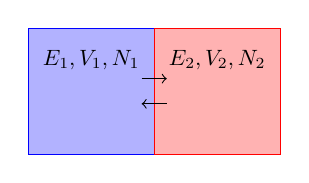
\begin{tikzpicture}[scale=0.8]
        % Primo quadrato
        \draw[blue,fill=blue!30] (0,0) rectangle (2,2);
        \node[scale=0.8]  at (1,1.5){$E_1,V_1,N_1$};
        
        % Secondo quadrato attaccato al primo
        \draw[red,fill=red!30] (2,0) rectangle (4,2) ;
        \node[scale=0.8] at (3,1.5){$E_2,V_2,N_2$};

        \draw[->] (1.8,1.2) -- (2.2,1.2);
        \draw[<-] (1.8,.8) -- (2.2,0.8);
      \end{tikzpicture}
    \small The two systems that we are studying.      
}
Let's consider two systems characterized by $(E_1,V_1,N_1)$ and $(E_2,V_2,N_2)$. These two systems can exchange energy and thus together the form an isolated system. We will assume that the total energy of the system is the sum of the energies of the two, because in the thermodynamic limit every energy contribution due to interaction on the surface of contact will be negligible.\\The phase space of the whole system is described by $(q_i^1,p_i^1,q_j^2,p_j2)$ (the coordinates of one system and of the other one) and will have a volume element $d\Gamma=d\Gamma_1d\Gamma_2$.\\
The area of the surface of constant energy ($E$) in the total phase space is:
\begin{align*}
    \omega(E)&=\int_{\mathcal{M} }d\Lambda_1d\Lambda_2\delta(\mathcal{H}-E)\\&=\int dE_1\int dS_{E_1}\int dE_2\int dS_{E_2}\delta(\mathcal{H}-E)\\&=\int dE_1\int dE_2\delta(\mathcal{H}-E)\omega(E_1)\omega(E_2)\\&=\int_0^{E} dE_1\omega(E_1)\omega(E-E_1)\leq\max_{E_1\in[0,E]}\omega(E_1)\omega(E-E_1)E.
\end{align*}
Defining $E^*$ as the energy that maximize the above expression:
\begin{equation*}
    \omega(E)\Delta E\leq\omega(E_1^*)\omega(E-E_1^*)E\Delta E.
\end{equation*}
Now, for some $\Delta E$ it is true:
\begin{equation*}
    \Delta E \omega(E_1^*)\omega(E-E_1^*)\leq\omega(E),
\end{equation*}
therefore
\begin{equation*}
    (\Delta E)^2 \omega(E_1^*)\omega(E-E_1^*)\leq\Delta E\omega(E)\leq\omega(E_1^*)\omega(E-E_1^*)E\Delta E.
\end{equation*}
Considering the volume $\Gamma(E)=\Delta E\omega(E)$ the above inequality reads:
\begin{equation*}
    \Gamma_1(E_1^*)\Gamma_2(E-E_1^*)\leq\Gamma(E)\leq\Gamma_1(E_1^*)\Gamma_2(E-E_1^*)\frac{E}{\Delta E},
\end{equation*}
taking the logarithm of all the sides:
\begin{equation*}
    \log\Gamma_1(E_1^*)+\log\Gamma_2(E-E_1^*)\leq\log\Gamma(E)\leq\log\Gamma_1(E_1^*)+\log\Gamma_2(E-E_1^*)+\log\frac{E}{\Delta E}.
\end{equation*}
In the thermodynamic limit the term $\log\frac{E}{\Delta E}\rightarrow0$, thus at equilibrium the entropy of each system is maximum and the total entropy\footnote{Since we are at the thermodynamic limit we cannot use the entropy because it would be infinite, we thus use the entropy per unit volume.} is given by the sum of the entropy of each subsystem:
\begin{equation*}
    s(E)=s_1(E_1^*)+s_2(E_2^*).
\end{equation*} 
If we consider a variation of energy of the subsystems $\delta E_1=-\delta E_2$ that will cause a variation of the volume $\Gamma$, this last one must be zero at equilibrium:
\begin{align*}
    &\delta \Lambda= \frac{\partial \Gamma_1}{\partial E_1}\bigg|_{E_1^*}\delta E_1 \Gamma_2+\Gamma_1\frac{\partial \Gamma_2}{\partial E_2}\bigg|_{E_2^*}\delta E_2=0\\&
    \Rightarrow\bigg(\frac{1}{\Gamma_1}\frac{\partial \Gamma_1}{\partial E_1}\bigg|_{E_1^*}-\frac{1}{\Gamma_2}\frac{\partial \Gamma_2}{\partial E_2}\bigg|_{E_2^*}\bigg)\delta E_1=0
    \\&
    \Rightarrow\frac{\partial \log\Gamma_1}{\partial E_1}\bigg|_{E_1^*}=\frac{\partial \log\Gamma_2}{\partial E_2}\bigg|_{E_2^*}\bigg. 
\end{align*}
This shows that the microcanonical entropy we have defined, at equilibrium, plays the same role as the thermodynamic entropy, since $\frac{\partial S}{\partial E}\big|_{V,N}=\frac{1}{T}$.\\

Lastly, we can show that we can evaluate the entropy in two other ways: first using that in the microcanonical case $\Gamma(E)=\Delta E\omega(E)$ with some arbitrary small $\delta E$, we get
\begin{equation*}
    S=k_B\log\Gamma=k_B\log\omega.
\end{equation*}
Given this observation we can prove that the \textbf{Boltzmann universal formula} holds:
\begin{equation*}
    \big<\log\rho_{mc}\big>=\int_{\mathcal{M} } d\Gamma\rho_{mc} \log\rho_{mc}=\int_{S_E}dS_E \frac{\log\frac{1}{\omega(E)}}{\omega(E)}=\log\frac{1}{\omega(E)}\int_{S_E} \frac{dS_E}{\omega(E)}=-\frac{S}{k_B}.
\end{equation*}
\begin{example}[The ideal gas]
    We will now study, as an example, the ideal gas. As ideal gas we mean $N$ classical, indistinguishable, non-interacting particles in a finite volume $V$. The Hamiltonian is $\mathcal{H} =\sum_{i=1}^n\frac{p_i^2}{2m}$.\\ In order to calculate $\omega(E)$ we can use that, given $\Sigma(E)$ the volume in phase space whose points have energy lower than $E$, $\omega(E)=\frac{\partial \Sigma}{\partial E}$.
    \begin{align*}
        \Sigma(E)&=\int_{0<\mathcal{H} <E}\frac{\Pi^N_id^3q_id^3p_i}{h^{3N}}=\frac{1}{h^{3N}}\int_{V}\Pi^N_id^3q_i\int_{0<\sum p_i^2<2mE}\Pi^N_id^3p_i\\&=\frac{V^N}{h^{3N}}\Omega_{3N}(\sqrt{2mE}),
    \end{align*} 
    where $\Omega_{3N}(\sqrt{2mE})$ is the volume of a $3N$-dimensional sphere with radius $\sqrt{2mE}$, ad $h$ is some constant that has the dimension of an action. Ignoring the all the multiplicative constants $\Omega_{3N}(\sqrt{2mE})\propto (2mE)^{\frac{3}{2}N}$, thus:\begin{equation*}
       \frac{\partial\Omega}{\partial E}=k\frac{3N}{2}(2mE)^{\frac{3N}{2}-1}2m=\frac{3N}{2E}\Omega\ \Rightarrow\ \omega(E)= \frac{\partial\Sigma}{\partial E}=\frac{3N}{2E}\Sigma.
    \end{equation*}
    From this result we can observe that, in the thermodynamic limit $N\rightarrow\infty$:
    \begin{equation*}
        \frac{\log\omega(E)}{N}=\frac{\log\Sigma(E)}{N}+\frac{\log\frac{3N}{2E}}{N}\rightarrow\frac{\log\Sigma(E)}{N}.
    \end{equation*}
    This relation, we have proved just for the ideal gas, holds for every system.\\
    In this way we can calculate entropy using $\Sigma(E)$; to evaluate it we need the explicit form of $\Omega_{3N}(\sqrt{2mE})=\frac{(2\pi mE)^{\frac{3N}{2}}}{N\Gamma(\frac{3N}{2})}$, thus we get:
    \begin{equation*}
        S=k_B\log\Sigma(E)=k_B\bigg\{N\log V\bigg(\frac{2\pi mE}{h^2}\bigg)^{\frac{3}{2}}-\log N-\log\Gamma\bigg(\frac{3N}{2}\bigg)+\log\frac{2}{3}\bigg\}.
    \end{equation*}
    Considering the thermodynamic limit and the Stirling's approximation it reads:
    \begin{equation*}
        S=k_B\bigg\{N\log V\bigg(\frac{2\pi mE}{h^2}\bigg)^{\frac{3}{2}}-\frac{3N}{2}\log\frac{3N}{2}+\frac{3N}{2}\bigg\}=\frac{3}{2}Nk_B+Nk_B\log V\bigg(\frac{4\pi mE}{3Nh^2}\bigg)^{\frac{3}{2}}.
    \end{equation*}
    We should notice that the entropy we obtained in not extensive, this is due to the fact that we are not considering the indistinguishability of the particle, and so we are double counting some states in the integration process. Dividing $\Sigma$ by $N!$ we discard all the double counted states and so (using Stirling' approximation) we obtain:
    \begin{equation*}
        S=\frac{5}{2}Nk_B+Nk_B\log \frac{V}{N}\bigg(\frac{4\pi mE}{3Nh^2}\bigg)^{\frac{3}{2}},
    \end{equation*}
    which is now extensive.\\From the entropy we have obtained we can find the internal energy:
    \begin{equation*}
        \frac{1}{T}=\frac{\partial S}{\partial E}\bigg|_{V,N}=\frac{3}{2}\frac{Nk_B}{E}\quad\Rightarrow\quad E=\frac{3}{2}K_B T;
    \end{equation*}
    and the state equation:
    \begin{equation*}
        \frac{P}{T}=\frac{\partial S}{\partial V}\bigg|_{E,N}=\frac{Nk_B}{V}\quad\Rightarrow\quad PV=NK_B T.
    \end{equation*}
\end{example}
\section{The canonical ensemble}
We now want to study systems that can exchange energy, and thus they don't have a fixed one. Those systems are better studied by the \textbf{canonical ensemble}.\\
\marginnote{
    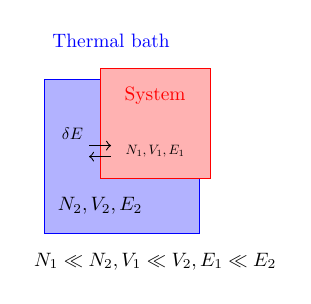
\begin{tikzpicture}[scale=0.7]
        % Quadrato esterno rosso
        \draw[blue, fill=blue!30,scale=0.7] (0,0) rectangle (4,4);
        \node[scale=0.7] at(1,.5){$N_2,V_2,E_2$};
        \node[blue,scale=0.7] at(1.2,3.5){Thermal bath};
        
        % Quadrato interno blu
        \draw[red, fill=red!30] (1,1) rectangle (3,3);
        \node[scale=0.7,scale=0.7] at(2,1.5){$N_1,V_1,E_1$};
        \node[red,scale=0.7] at(2,2.5){System};
        \node[scale=0.7] at(2,-.5){$N_1\ll N_2,V_1\ll V_2,E_1\ll E_2$};
        \draw[->] (.8,1.6)node[scale=.6,anchor=south east]{$\delta E$} -- (1.2,1.6);
        \draw[<-] (.8,1.4) -- (1.2,1.4);
      \end{tikzpicture}
     \small A simple sketch of the system and the thermal bath.
}
In order to study such systems we will introduce a thermal bath (denoted by the numer $2$), much bigger than our system (denoted by the number $1$).  The two systems can exchange energy one to the other, but together they form an isolated system. These two are at thermal equilibrium ($T_1=T_2=T$). In this way we can tackle this problem using the microcanonical approach we have just developed in the last section \ref{sec:MicroCan}. The total system will have energy $E=E_1+E_2$ and thus the microcanonical probability distribution will be:
\begin{equation*}
    \rho_{mc}=\frac{\delta(\mathcal{H}_1+\mathcal{H}_2-E_1-E_2)}{\omega(E_1+E_2)}.
\end{equation*}
We now want to find the marginal distribution depending on just the variables of our system. To do so we have to integrate over the phase space of the thermal bath:
\begin{equation*}
    \int_{\mathcal{M}_2 }\Pi^{N_2}_j dq^{(2)}_jdp^{(2)}_j\rho_{mc}(q^{(1)}_i,p^{(1)}_i,q^{(2)}_j,p^{(2)}_j)=\int_{\mathcal{M}_2 }\Pi^{N_2}_j dq^{(2)}_jdp^{(2)}_j\frac{\delta(\mathcal{H}_1+\mathcal{H}_2-E_1-E_2)}{\omega(E_1+E_2)},
\end{equation*}
the Dirac's delta fixes the energy of the thermal bath in terms of the energy of our system. Recalling that $S=k_B\log\omega$, the integral above results in:
\begin{equation*}
    \Rightarrow\quad \frac{\omega_2(E_2=E-E_1)}{\omega(E)}=\frac{1}{\omega(E)}\exp\bigg\{\frac{1}{k_B}S_2(E-E_1)\bigg\}.
\end{equation*}
We now recall that the thermal bath is built as "bigger" than the system, mathematically we mean $E_1\ll E_2$, therefore $E_1\ll E$. This construction let us Taylor expand the exponential with respect to $E_1$, since $\frac{\partial S}{\partial E}=\frac{1}{T}$:
\begin{equation*}
    \frac{1}{\omega(E)}\exp\bigg\{\frac{1}{k_B}\bigg[S_2(E)-\frac{\partial S_2}{\partial E}E_1\bigg]\bigg\}=\frac{\exp\big\{\frac{S_2(E)}{k_B}\big\}}{\omega(E)}\exp\bigg\{-\frac{E_1}{k_BT}\bigg\}.
\end{equation*}
We have found the marginal probability distribution of our system, called canonical distribution. Since we don't want always have to use the entropy and energy of the bath, we put all the terms depending on those in a constant that we can evaluate using the normalization of the function.
\begin{equation}\label{CanonicalDistribution}
    \rho_C(q_i,p_i)=\frac{e^{-\beta\mathcal{H} }}{Z_N},\qquad\qquad\beta=\frac{1}{k_BT},\quad Z_N=\int_{\mathcal{M} ^N}d\Omega\ e^{-\beta\mathcal{H} }.
\end{equation} 
We could think that $Z_N$, called the \textbf{partition function}, is just a constant (indeed it is a constant with respect of our distribution) but we should notice that it is dependent on the temperature of the system, due to $\beta$, the number of particles of the system and the volume of the system, due to the integration over $\mathcal{M}^N$. We will see that, for this reason, $Z_N$ is related to a thermodynamic potential that depends on the same variables.\\

Let's observe that, as we saw in the microcanonical framework, this approach over counts the states of the system, assuming that all the particles are always distinguishable (as in the lattice of a crystal). To solve this over counting we have to divide the volume element in phase space by a factor $N!$, in this way $Z_N\rightarrow\frac{Z_N}{N!}$.\\

Lastly, let's consider a system made up of different types of particles, each one with its hamiltonian:
\begin{equation*}
    N=\sum_{i}N_i,\qquad \mathcal{H} =\sum_i\mathcal{H}_i.
\end{equation*}
Given $\Omega_i$ the volume element of the phase space of the $i$-esim system (scaled to account indistinguishability and remove the dimension), the total partition function reads:
\begin{align*}
    Z_N&=\int_{\mathcal{M}^N}\Pi_id\Omega_i\ e^{-\beta\sum_i\mathcal{H}_i}=\bigg(\int_{\mathcal{M}^{N_1} }d\Omega_1e^{-\beta\mathcal{H}_1}\bigg)\bigg(\int_{\mathcal{M}^{N_2} }d\Omega_2e^{-\beta\mathcal{H}_2}\bigg)...\\&=\Pi_iZ_{N_i}.
\end{align*} 
This approach can be used to evaluate the partition function of a system of $N$ identical particle as $ Z_N=Z^N$, where $Z$ is the partition function of one single particle.
\subsection{Partition function and free energy}
As already mentioned, the partition function depends on $V,T,N$. There is a thermodynamic potential, the Helmholtz's free energy, which depends on the same variables. We will show that defining an arbitray function $F(T,V,N)$, such that
\begin{equation*}
    Z_N(T,V)\triangleq e^{-\beta F(T,V,N)},
\end{equation*}
this function behave exactly as the Helmholtz's free energy.\\

First, from the above definition, the normalization condition of Eq. \eqref{CanonicalDistribution} reads
\begin{equation*}
    1=\int d\Omega \frac{e^{-\beta\mathcal{H} }}{Z_N}=\int d\Omega\ e^{-\beta(\mathcal{H}-F)}, 
\end{equation*}
differentiating this expression with respect to $\beta$ we get:
\begin{align*}
    0&=\int d\Omega \frac{e^{-\beta\mathcal{H} }}{Z_N}=\int d\Omega \frac{\partial}{\partial\beta}e^{-\beta(\mathcal{H}-F)}=\int d\Omega\bigg[-(\mathcal{H} -F)+\beta\frac{\partial F}{\partial\beta}\bigg] e^{-\beta(\mathcal{H}-F)}\\&=-\int d\Omega \frac{e^{-\beta\mathcal{H} }}{Z_N}\mathcal{H} +F+\beta\frac{\partial F}{\partial\beta}=-E+F+\beta\frac{\partial F}{\partial\beta}\\
    &\Rightarrow\ E=F+\beta\frac{\partial F}{\partial\beta}=F-T\frac{\partial F}{\partial T}.
\end{align*}
If $F$ is the Helmholtz's free energy we should recall the relation
\begin{equation*}
    \frac{\partial F}{\partial T}=\frac{F-E}{T}=-S,
\end{equation*}
therefore, using the Boltzmann's universal formula as definition of entropy:
\begin{align*}
    S&=-k_B\big<\log\rho_C\big>=-k_B\int d\Omega\ \rho_C\log\rho_C=-k_B\int d\Omega\ \rho_C\log\frac{e^{-\beta\mathcal{H}} }{Z_N}\\&=-k_B\int d\Omega\ \rho_C\big(-\beta\mathcal{H} -\log Z_N \big)=\frac{E}{T}+k_B\frac{\beta}{\beta}\log Z_N\\&=\frac{E}{T}+\bigg(-\frac{1}{T}\bigg)\bigg(-\frac{1}{\beta}\log Z_N\bigg)=\frac{E}{T}-\frac{F}{T},
\end{align*}
which shows that these two definitions of the free energy and entropy lead to the same relations that holds in thermodynamic.\\

From these caluclation we have found the follwing relations, that can be used to easily get thermodynamic variables from the partition function:
\begin{align*}
    F&=-\frac{1}{\beta}\log Z_N,\\
    E&=\int d\Omega\ \mathcal{H} \frac{e^{-\beta\mathcal{H} }}{Z_N}=-\frac{1}{Z_N}\int d\Omega\ \frac{\partial}{\partial\beta} e^{-\beta\mathcal{H} }=-\frac{1}{Z_N}\frac{\partial Z_N}{\partial\beta}=-\frac{\partial\log Z_N}{\partial\beta}.
\end{align*} 
\subsection{Equipartition theorem}
Using the canonical framework it is possible to derive a really useful result that can help to study systems without the need of determining the whole partition function. This is the \textbf{equipartition theorem} which allow to calculate the internal energy of a system just by studying its hamiltonian. We will now illustrate its generalized form.
\begin{theorem}[Generalized equipartition theorem]\label{thm:GeneralizedEquipartition}
    Let $\xi_1\in[a,b]$ be one of the canonical coordinates or momenta and $\xi_j\ j>1$ denotes all the others.\\ If holds that $\int \Pi_{j\neq1}d\xi_j[\xi_1e^{-\beta\mathcal{H} }]_a^b=0$ then:
    \begin{equation}
        \bigg<\xi_1\frac{\partial\mathcal{H} }{\partial \xi_1}\bigg>=k_BT.
    \end{equation}
\end{theorem}
\begin{proof}
    We will start by the normalization condition of the canonical distribution:
    \begin{equation*}
        1=\int d\Omega\frac{e^{-\beta\mathcal{H} }}{Z_N}=\frac{1}{Z_N}\int d\xi_1(\Pi_{j\neq1}d\xi_j) e^{-\beta\mathcal{H}}.
    \end{equation*}
    Since $\frac{d}{d\xi_1}\big[\xi_1\exp(-\beta\mathcal{H} )\big]=\exp(-\beta\mathcal{H} )-\beta\xi_1\exp(-\beta\mathcal{H} )\frac{\partial\mathcal{H} }{\partial\xi_1}$ we can integrate by parts with respect to $\xi_1$:
    \begin{align*}
        1&=\frac{1}{Z_N}\int(\Pi_{j\neq1}d\xi_j)\bigg(d\big[\xi_1e^{-\beta\mathcal{H}}\big]+\beta\xi_1e^{-\beta\mathcal{H}}\frac{\partial\mathcal{H} }{\partial\xi_1}d\xi_1\bigg) \\
        &=\frac{1}{Z_N}\int(\Pi_{j\neq1}d\xi_j)\big[\xi_1e^{-\beta\mathcal{H}}\big]_a^b+\frac{\beta}{Z_N}\int(\Pi_{j\neq1}d\xi_j)\xi_1e^{-\beta\mathcal{H}}\frac{\partial\mathcal{H} }{\partial\xi_1}d\xi_1.
    \end{align*}
    The fist integral is zero by hypothesis and the second correspond to the mean value of $\xi_1\frac{\partial\mathcal{H} }{\partial \xi_1}$:
    \begin{align*}
        \frac{1}{\beta}=k_BT=\int d\Omega\frac{e^{-\beta\mathcal{H} }}{Z_N}\xi_1\frac{\partial\mathcal{H} }{\partial \xi_1}=\bigg<\xi_1\frac{\partial\mathcal{H} }{\partial \xi_1}\bigg>
    \end{align*}
\end{proof}
The standard equipartition theorem, can be obtained as corollary of the previous theorem. 
\begin{corollary}[Equipartition theorem]\label{thm:equiPart}
    The internal energy of a system has a $\frac{k_BT}{2}$ contribute for each quadratic term that appears in the hamiltonian.
\end{corollary}
\begin{proof}
    Let's consider a quadratic hamiltonian in $\xi_1$:
    \begin{equation*}
        \mathcal{H} =A\xi_1^2+G(\xi_2,\xi_3,\dots),
    \end{equation*}
    with $G$ arbitrary function. Clearly $\xi_1$ satisfies the hypothesis of the generalized equipartition theorem \ref{thm:GeneralizedEquipartition}, thus we can calculate:
    \begin{equation*}
        k_BT=\bigg<\xi_1\frac{\partial\mathcal{H} }{\partial \xi_1}\bigg>=\big<\xi_12A\xi_1\big>\quad \Rightarrow\quad \big<A\xi_1^2\big>=\frac{k_BT}{2}.
    \end{equation*} 
\end{proof}
\begin{example}[The energy of the ideal gas]
    As we already discussed, an ideal gas is made up of non-interacting classical and indistinguishable particles. Therefore, its hamiltonian is the sum of $N$ free particle hamiltonian:
    \begin{equation*}
        \mathcal{H}=\sum_i^N\frac{\vec p^2_i}{2m}.
    \end{equation*}
    Using the equipartition theorem \ref{thm:equiPart} we then get that the internal energy of the system is $E=\frac{3}{2}Nk_BT$. The same result can be obtained studying the partition function:
    \begin{align*}
        Z_N&=\frac{Z_1^N}{N!}\\
        Z_1&=\frac{1}{h^3}\int_V d^3q\int_{\mathbb{R}^3}d^3p\ e^{-\beta\frac{\vec{ p}^2}{2m}}=\frac{V}{h^3}\int_{\mathbb{R}^3}d^3p\ e^{-\beta\frac{\vec{ p}^2}{2m}}\\&=\frac{V}{h^3}\bigg(\int_{-\infty}^{+\infty}d^3p\ e^{-\beta\frac{ p^2}{2m}}\bigg)^3=\frac{V}{h^3}\bigg(\frac{2m\pi}{\beta}\bigg)^{\frac{3}{2}}=V\bigg(\frac{2m\pi k_BT}{h^2}\bigg)^{\frac{3}{2}},\\
        Z_N&=\frac{V^N}{N!}\bigg(\frac{2m\pi k_BT}{h^2}\bigg)^{\frac{3}{2}N},\\
        E&=-\frac{\partial \log Z_n}{\partial\beta}=\frac{3}{2}Nk_BT.
    \end{align*}

\end{example}
\begin{example}[The energy of the ultrarelativistic gas]
    We can consider an ultra relativistic gas as a gas of relativistic particles whose kinetic energy is much bigger than the energy due to the rest mass, thus this last can be neglected:
    \begin{equation*}
        \mathcal{H}= \sum_i^N\sqrt{c^2\vec p_i^2+m^2c^4}\approx\sum_i^N c|\vec p_i|.
    \end{equation*}
    Since the hamiltonian isn't quadratic, we have to use the generalized equipartition theorem \ref{thm:GeneralizedEquipartition}: notice that this hamiltonian satisfy its hypothesis because it is always positive, and thus $[|\vec p_i|\exp(-\beta\sum_i^N c|\vec p_i|)]_{-\infty}^{+\infty}=0$. From the theorem we get:
    \begin{equation*}
        \bigg<p_{i,x}\frac{\partial\mathcal{H} }{\partial p_{i,x}}\bigg>=\bigg<p_{i,x}c\frac{p_{i,x}}{|\vec p_i|}\bigg>=k_BT.
    \end{equation*}
    Summing this expression over all the components of the momentum of one particle:
    \begin{equation*}
        3k_BT=\bigg<c\frac{p^2_{i,x}+p^2_{i,y}+p^2_{i,z}}{|\vec p_i|}\bigg>=\bigg<c\frac{p^2_{i}}{|\vec p_i|}\bigg>=\big<c|\vec p_i|\big>.
    \end{equation*}
    Lastly, summing over all the particles we get:
    \begin{equation*}
        \sum_i^n\big<c|\vec p_i|\big>=\big<\mathcal{H} \big>=3Nk_BT.
    \end{equation*}
\end{example}
\begin{example}[1-D solid]
    As the last example of the canonical ensemble framework we will discuss the case of a $1$-D lattice of atoms, forming a sort of solid. Each atom is fixed to its own equilibrium position, and can oscillate around it. The lattice is therefore created by harmonic interactions between neighbors atoms, resulting in a total hamiltonian of the form:
    \begin{equation*}
        \mathcal{H} =\sum_{i}\bigg(\frac{p_i^2}{2m}+\frac{m\omega^2}{2}q_i^2\bigg).
    \end{equation*}
    We will find the total partition function by studying the single particle system:
    \begin{equation*}
        Z_1=\int_{-\infty}^{+\infty}dq\ e^{-\beta\frac{m\omega^2}{2}q^2} \int_{-\infty}^{+\infty}dp\frac{e^{-\beta\frac{p_i^2}{2m}}}{h}=\frac{\pi}{h}\sqrt{\frac{2k_BT}{m\omega^2}2mk_BT}=\frac{2\pi k_BT}{\omega h}. 
    \end{equation*}
    We must notice that every single particle is not indistinguishable from the others, because the lattice structure gives to each particle a precise position in it, thus we can distinguish two particles by their positions. The total partition function is therefore:
    \begin{equation*}
        Z_N=Z_1^N=\bigg(\frac{2\pi k_BT}{\omega h}\bigg)^N.
    \end{equation*}
    We can now obtain the main thermodynamic variables:
    \begin{align*}
        F&=-\frac{1}{\beta}\log Z_n=-Nk_BT\log\bigg(\frac{2\pi k_BT}{\omega h}\bigg)\\
        E&=-\frac{\partial\log Z_N}{partial\beta}=Nk_BT,\\
        S&=\frac{E-F}{T}=Nk_BT+Nk_BT\log\bigg(\frac{2\pi k_BT}{\omega h}\bigg)\\
        P&=-\frac{\partial F}{\partial V}\bigg|_{T,N}=0.
    \end{align*}
    Let's observe that the pressure of this system is always zero: this can be interpreted as a consequence of the infinite volume of this system (since we have integrated over the whole configuration space)-
\end{example}
\section{Grand canonical ensemble}
In this section we will discuss the framework used to study open systems. In this way we will have to account for a non-fixed number of particles. For this reason, the distribution describing our system is defined over each phase space of $n$ particles, going from $1$ to $\infty$.\\

We will derive the grand canonical partition function by studying our system (denoted by $(1)$) embedded (at equilibrium) in a thermal bath (denoted by $(2)$) such that the whole universe (system plus bath) is a closed system, therefore described by the canonical partition function.
\marginnote{
    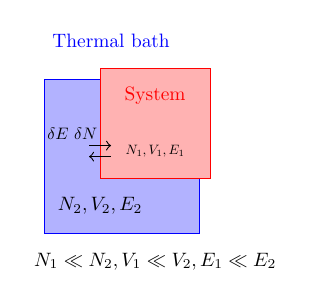
\begin{tikzpicture}[scale=0.7]
        % Quadrato esterno rosso
        \draw[blue, fill=blue!30,scale=0.7] (0,0) rectangle (4,4);
        \node[scale=0.7] at(1,.5){$N_2,V_2,E_2$};
        \node[blue,scale=0.7] at(1.2,3.5){Thermal bath};
        
        % Quadrato interno blu
        \draw[red, fill=red!30] (1,1) rectangle (3,3);
        \node[scale=0.7,scale=0.7] at(2,1.5){$N_1,V_1,E_1$};
        \node[red,scale=0.7] at(2,2.5){System};
        \node[scale=0.7] at(2,-.5){$N_1\ll N_2,V_1\ll V_2,E_1\ll E_2$};
        \draw[->] (.8,1.6)node[scale=.6,anchor=south ]{$\delta E\ \delta N\quad\quad$} -- (1.2,1.6);
        \draw[<-] (.8,1.4) -- (1.2,1.4);
      \end{tikzpicture}
     \small A simple sketch of the system and the thermal bath.
}
\begin{equation*}
    \rho_c(q_i^{(1)},p_i^{(1)},q_j^{(2)},p_j^{(2)})=\frac{e^{-{\beta(\mathcal{H}_1+\mathcal{H}_2)}}}{Z_N}.
\end{equation*}
We can fix the number of particles in each system in order to integrate over the phase space of the bath and thus get the marginal distribution of our system (with $N_1$ particles). Doing this integration we will assume the normalization constant of the distribution of the system to be $\frac{N!}{N_1!N_2!}$, and we will later check that our assumption was the right one.
\begin{align*}
    \rho_{gc}&=\frac{N!}{N_1!N_2!}\int_{\mathcal{M}^{N_2}}\Pi_{j}dq_j^{(2)}\ dp_j^{(2)}\rho_c\\&=\frac{N!}{N_1!N_2!}\int_{\mathcal{M}^{N_2}}\Pi_{j}dq_j^{(2)}\ dp_j^{(2)}\frac{e^{-\beta\mathcal{H}_1}e^{-\beta\mathcal{H}_2}}{\int\ d\Gamma\ \exp(-\beta{\mathcal{H}_1+\mathcal{H}_2})}\frac{h^{dN}}{h^{dN}}\\&=\frac{Z_{N_2}}{Z_{N}}\frac{e^{-\beta\mathcal{H}_1}}{N_1!h^{dN_1}}.
\end{align*}
This is the grand canonical distribution for our system. We will now check our assumption by integrating it over the phase space of the system with $N_1$ particles and then summing up all the contribution of all the integrals with different numbers of particles (up to the total number of particles of the universe). We expect that the result of this operation should be equals to $1$.
\begin{equation*}
    \sum_{N_1=0}^{N}\int_{\mathcal{M}^{N_1}}\rho_{gc}d\Omega_{N_1}=\sum_{N_1=0}^{N}\frac{Z_{N_2}}{Z_{N}}\int_{\mathcal{M}^{N_1}}\frac{e^{-\beta\mathcal{H}_1}}{N_1!h^{dN_1}}d\Omega_{N_1}=\sum_{N_1=0}^{N}\frac{Z_{N_2}Z_{N_1}}{Z_{N}}.
\end{equation*}
This expression doesn't add up to one, since each partition function is integrated over different phase spaces: this problem is solved by considering the bath infinitely large (in the thermodynamic limit). We firstly define
\begin{equation*}
    \phi(q)=\int_{\mathbb{R} ^{dN_1}}\Pi_i dp_i^{(1)}\int_{\mathbb{R} ^{dN_2}}\Pi_j dp_j^{(2)}e^{-\beta(\mathcal{H}_1+\mathcal{H} _2)},
\end{equation*}  
in this way the above sum reads:
\begin{align*}
    \sum_{N_1=0}^{N}\int_{\mathcal{M}^{N_1}}\rho_{gc}d\Omega_{N_1}&=\sum_{N_1=0}^{N} \frac{N!}{N_1!N_2!}\frac{\int_{\mathcal{M}^{N_1}}d\Gamma_1 e^{-\beta\mathcal{H}_1}\int_{\mathcal{M}^N_{N_2}}d\Gamma_2 e^{-\beta\mathcal{H}_2}}{\int\ d\Gamma\ \exp(-\beta{\mathcal{H}_1+\mathcal{H}_2})} 
    \\&=\sum_{N_1=0}^{N} \frac{N!}{N_1!N_2!}\frac{\int_{V_1}\Pi_i dq_i^{(1)}\int_{V_2}\Pi_j dq_j^{(2)}\phi(q)}{\int_{V_1+V_2}\Pi_i dq_i^{(1)}\int_{V_1+V_2}\Pi_j dq_j^{(2)}\phi(q)}.
\end{align*}
We define $\big<\phi\big>_{V}$ as the mean value of $\phi$ over the volume of integration, normalized by dividing by such volume, in this way the sum reads:
\begin{equation*}
    \sum_{N_1=0}^{N}\int_{\mathcal{M}^{N_1}}\rho_{gc}d\Omega_{N_1}=\sum_{N_1=0}^{N}\frac{V_1^{N_1}V_2^{N_2}}{(V_1+V_2)^{N_1+N_2}}\frac{\big<\phi\big>_{V_1V_2}}{\big<\phi\big>_{V}}=\sum_{N_1=0}^{N}\bigg(\frac{V_1}{V}\bigg)^{N_1}\bigg(\frac{V_2}{V}\bigg)^{N_2}\frac{\big<\phi\big>_{V_1V_2}}{\big<\phi\big>_{V}}.
\end{equation*}
In the thermodynamic limit the volumes go to infinity, as for the number of particles, thus the tho averages tend to the same limit, we then get:
\begin{equation*}
    \lim_{V\rightarrow\infty} \sum_{N_1=0}^{N}\int_{\mathcal{M}^{N_1}}\rho_{gc}d\Omega_{N_1}\approx\lim_{N\rightarrow\infty}\sum_{N_1=0}^{N}\bigg(\frac{V_1}{V}\bigg)^{N_1}\bigg(\frac{V_2}{V}\bigg)^{N_2}=\lim_{N\rightarrow\infty}\bigg(\frac{V_1+V_2}{V}\bigg)^N=1
\end{equation*}
Therefore, in the thermodynamic limit our initial assumption holds.\\

Lastly we need to remove all the explicit dependencies by the variables of the thermal bath, using the definition of the Gibb's free energy, given for the canonical ensemble, we can get:
\begin{equation*}
    \frac{Z_{N_2}}{Z_N}= \exp\bigg\{-\beta F(T,N-N_1,V-V_1)+\beta F(T,N,V)\bigg\}\approx \exp\bigg\{\beta\frac{\partial F}{\partial N}N_1+\beta\frac{\partial F}{\partial V}V_1\bigg\},
\end{equation*}
in which we have used Taylor expansion to the first order, considering the bath larger than our system. If we define $\mu=\frac{\partial F}{\partial N}$, the chemical potential, and reminding that from classical thermodynamic $P=-\frac{\partial F}{\partial V}$, the grand canonical distribution reads:
\begin{equation*}
    \rho_{gc}=\frac{e^{-\beta\mathcal{H}_1 }}{N_1!h^{dN_1}}e^{\beta\mu N_1}e^{-\beta PV_1}.
\end{equation*}
We can now remove the label of the system and define the \textbf{fugacity}
\begin{equation*}
    z=e^{\beta N}
\end{equation*}
and the \textbf{grand potential}
\begin{equation*}
    \Omega=-PV=E-TS-\mu N,
\end{equation*}
using the normalization condition we get:
\begin{align*}
    1&=\sum_{N=0}^{\infty}\int_{\mathcal{M}^N}d\Omega_Ne^{-\beta\mathcal{H}}e^{\beta\mu N}e^{-\beta PV}=e^{-\beta PV}\sum_{N=0}^{\infty}e^{\beta\mu N}\int_{\mathcal{M}^N}d\Omega_Ne^{-\beta\mathcal{H}}\\&=e^{\Omega}\sum_{N=0}^{\infty}z^{N}Z_N.
\end{align*}
Defining the \textbf{grand canonical partition function}
\begin{equation}
    \label{GCPartitionFunc}\mathcal{Z} =\sum_{N=0}^{\infty}z^{N}Z_N\quad\Rightarrow\quad \Omega=-\frac{\log\mathcal{Z} }{\beta},
\end{equation}
the grand canonical distribution reads:
\begin{equation}
    \label{GrandCanonicalDistribution} \rho_{gc}=\frac{e^{-\beta\mathcal{H} }e^{\beta\mu N}}{\mathcal{Z}}.
\end{equation}
Having the full distribution allows us to calculate means values of the mechanical variables of the system. These can be expressed in terms of the canonical means:
\begin{align*}
    <f>_{gc}&=\sum_{N=0}^{\infty}\int_{\mathcal{M}^N}d\Omega_N\frac{e^{-\beta\mathcal{H} }e^{\beta\mu N}}{\mathcal{Z}}f(q_i,p_i)=\frac{1}{\mathcal{Z} }\sum_{N=0}^{\infty}Z_Ne^{\beta\mu N}\int_{\mathcal{M}^N}d\Omega_N\frac{e^{-\beta\mathcal{H} }}{Z_N}f(q_i,p_i)\\&=\frac{1}{\mathcal{Z} }\sum_{N=0}^{\infty}Z_Nz^N<f>_c.
\end{align*}
We now calculate all the main thermodynamic variables:
\begin{align*}
    E&=<\mathcal{H} >=\sum_{N=0}^{\infty}\int_{\mathcal{M}^N}d\Omega_N\frac{e^{-\beta\mathcal{H} }e^{\beta\mu N}}{\mathcal{Z}}\mathcal{H} =\frac{-1}{\mathcal{Z}}\sum_{N=0}^{\infty}z^N\int_{\mathcal{M}^N}d\Omega_N\frac{\partial}{\partial\beta}e^{-\beta\mathcal{H} }\\&=\frac{-1}{\mathcal{Z}}\frac{\partial}{\partial\beta}\sum_{N=0}^{\infty}z^N\int_{\mathcal{M}^N}d\Omega_Ne^{-\beta\mathcal{H} }\bigg|_{z\text{ fixed}}=-\frac{1}{\mathcal{Z}}\frac{\partial\mathcal{Z}}{\partial\beta}\bigg|_{z\text{ fixed}},\\
    <N>&=\sum_{N=0}^{\infty}\int_{\mathcal{M}^N}d\Omega_N\frac{e^{-\beta\mathcal{H} }e^{\beta\mu N}}{\mathcal{Z}}N=\sum_{N=0}^{\infty}e^{\beta\mu N}N\frac{Z_N}{\mathcal{Z} }\int_{\mathcal{M}^N}d\Omega_N\frac{e^{-\beta\mathcal{H} }}{Z_N}\\&=\sum_{N=0}^{\infty}e^{\beta\mu N}N\frac{Z_N}{\mathcal{Z} }=\frac{1}{\mathcal{Z} }\sum_{N=0}^{\infty}z^NNZ_N=\frac{z}{\mathcal{Z} }\frac{\partial}{\partial z}\sum_{N=0}^{\infty}z^NZ_N\bigg|_{\beta\text{ fixed}}\\&=\frac{z}{\mathcal{Z} }\frac{\partial\mathcal{Z} }{\partial z}\bigg|_{\beta\text{ fixed}}.
\end{align*}
Lastly we recover entropy using the Boltzmann's universal formula:
\begin{align*}
    S&=-k_B<\log\rho_{gc}>=-k_B\sum_{N=0}^{\infty}\int_{\mathcal{M}^N}d\Omega_N\frac{e^{-\beta\mathcal{H} }e^{\beta\mu N}}{\mathcal{Z}}[-\beta\mathcal{H} +\beta\mu N-\log\mathcal{Z} ]\\&=k_B\beta E-k_B\beta\mu<N>+k_B\log{\mathcal{Z}}\frac{\beta}{\beta}=\frac{E-\mu N-\Omega}{T}=S_{\text{Th}},
\end{align*}
which shows the constituency of all the definition of the thermodynamic variables.
\subsection{Van deer Waals' law}
We are going to derive the \textbf{Van deer Waals' law}, for real gasses, using the grand canonical framework. In order to do so we will need to approximate the grand canonical partition function using a so-called \textbf{virial expansion}.\\

Considering a small fugacity we will truncate the summation defining the partition function:
\begin{equation*}
    \mathcal{Z} =1+zZ_1+z^2Z_2+z^3Z_3+\dots\approx1+zZ_1.
\end{equation*}
Considering a gas of free particles, as we already derived, the partition function of the single particle is:
\begin{equation*}
    Z_1=V\bigg(\frac{2m\pi k_BT}{h^2}\bigg)^{\frac{3}{2}}=\frac{V}{\lambda^3_T}\quad \Rightarrow\quad \mathcal{Z} \approx1+z\frac{V}{\lambda_T^3}.
\end{equation*}
Since we are considering an approximation of the first order in $z$, we can evaluate the logarithm of $\mathcal{Z} $ truncating at the same order its Taylor's approximation
\begin{equation*}
    \log\mathcal{Z} \approx\log\bigg(1+z\frac{V}{\lambda_T^3}\bigg)\approx z\frac{V}{\lambda_T^3},
\end{equation*}
using the definitions given in the last section:
\begin{equation*}
    PV=\frac{\log\mathcal{Z} }{\beta}=z\frac{V}{\lambda_T^3\beta},\quad N=z\frac{\partial\log\mathcal{Z} }{\partial z}\bigg|_{\beta}=z\frac{V}{\lambda_T^3}\quad\Rightarrow\quad PV=k_BTN.
\end{equation*}
Therefore, the first order virial approximation results in the state equation of the ideal gas. We can notice that this also shows that a low fugacity (the limit that we are using for the approximation) corresponds to a very dilute gas.\\

Let's truncate such approximation at the second order, in order to do so we need to evaluate the partition function of two particles (that can interact):
\begin{align*}
    Z_2&=\frac{1}{2!}\int_{V}\int_{\mathbb{R} ^3}\frac{d^3q_1d^3p_1}{h^3}\int_{V}\int_{\mathbb{R} ^3}\frac{d^3q_2d^3p_2}{h^3}\exp\bigg\{-\beta\frac{\vec p^2_1+\vec p_2^2}{2m}-\beta U(|\vec q_1-\vec q_2|)\bigg\}\\&=\frac{1}{2\lambda_T^6}\int_{V}\int_Vd^3q_1d^3q_2e^{-\beta U(|\vec q_1-\vec q_2|)}\\
    &\text{Changing variables } \vec R=\frac{\vec q_1+\vec q_2}{2},\quad \vec r=\vec q_1-\vec q_2,\\
    &=\frac{1}{2\lambda_T^6}\int_{V}\int_Vd^3Rd^3r\ e^{-\beta U(|\vec r|)}=\frac{V}{2\lambda_T^6}\int_{V}d^3r\ e^{-\beta U(|\vec r|)}=\frac{V}{2\lambda_T^6}J_2(\beta).
\end{align*}
In our approximation the grand canonical partition function reads
\begin{equation*}
    \mathcal{Z} \approx1+z\frac{V}{\lambda_T^3}+z^2\frac{V}{2\lambda_T^6}J_2(\beta)
\end{equation*}
and thus 


